%%%%%%%%%%%%%%%%%%%%%%%%%%%%%%%%%%%%%%%%%%%%%%%%%%%%%%%%%%%%%%%%%%%%%%%%%%%%%%%%
%  Agents for Solving the Battleship Puzzle -- class presentation (10 minutes)
%  Artificial Intelligence 0406, Group 2, UNAM Facultad de Ingenieria
%
%  Compile:  pdflatex slides.tex   (twice)
%  It must be compiled INSIDE the report folder, because it reads
%  the images of  figuras/  and the data of  data/  (the same ones as the report).
%%%%%%%%%%%%%%%%%%%%%%%%%%%%%%%%%%%%%%%%%%%%%%%%%%%%%%%%%%%%%%%%%%%%%%%%%%%%%%%%
\documentclass[aspectratio=169,11pt]{beamer}
\usetheme{metropolis}
\metroset{sectionpage=none, subsectionpage=none, numbering=fraction, progressbar=frametitle, block=fill}

\usepackage[utf8]{inputenc}
\usepackage[english]{babel}
\usepackage{amsmath,amssymb}
\usepackage{booktabs}
\usepackage{graphicx}
\usepackage{caption}
\usepackage{pgfplots}
\pgfplotsset{compat=1.17, table/col sep=comma}
\usepgfplotslibrary{fillbetween}
\captionsetup{font=scriptsize, labelfont={scriptsize,bf}}

%%%%%%%%%%%%%%%%%%%%%%%%%%%%%%%%%%%%%%%%%%%%%%%%%%%%%%%%%%%%%%%%%%%%%%%%%%%%%%%%
%  Colours (the same ones as the report) and plot style
%%%%%%%%%%%%%%%%%%%%%%%%%%%%%%%%%%%%%%%%%%%%%%%%%%%%%%%%%%%%%%%%%%%%%%%%%%%%%%%%
\definecolor{cSRA}{HTML}{7F7F7F}    % SRA   = grey
\definecolor{cGBA}{HTML}{1F77B4}    % GBA   = blue
\definecolor{cABAOP}{HTML}{D62728}  % ABAOP = red
\definecolor{unam}{HTML}{06427A}    % dark blue of the application
\definecolor{sunglow}{rgb}{1.0, 0.8, 0.2}

\setbeamercolor{frametitle}{bg=unam}
\setbeamercolor{progress bar}{fg=sunglow}
\setbeamercolor{alerted text}{fg=unam}

\pgfplotsset{
  battle/.style={
    width=\linewidth, height=5.0cm, grid=major, grid style={gray!25},
    tick label style={font=\tiny}, label style={font=\scriptsize},
    title style={font=\scriptsize\bfseries},
    legend style={font=\tiny, fill=white, fill opacity=0.85, draw opacity=1, text opacity=1},
    every axis plot/.append style={line width=0.9pt}
  }
}

%%%%%%%%%%%%%%%%%%%%%%%%%%%%%%%%%%%%%%%%%%%%%%%%%%%%%%%%%%%%%%%%%%%%%%%%%%%%%%%%
%  \includegraphics that does NOT break the compilation while an image is missing:
%  it draws a grey box with the name of the file that has to be put in figuras/.
%%%%%%%%%%%%%%%%%%%%%%%%%%%%%%%%%%%%%%%%%%%%%%%%%%%%%%%%%%%%%%%%%%%%%%%%%%%%%%%%
\let\realincludegraphics\includegraphics
\renewcommand{\includegraphics}[2][]{%
  \IfFileExists{#2}%
    {\realincludegraphics[#1,height=0.58\textheight,keepaspectratio]{#2}}%
    {\fbox{\parbox[c][3.2cm][c]{0.85\linewidth}{\centering\color{gray}\ttfamily\scriptsize [figure to add: \detokenize{#2}]}}}}

%%%%%%%%%%%%%%%%%%%%%%%%%%%%%%%%%%%%%%%%%%%%%%%%%%%%%%%%%%%%%%%%%%%%%%%%%%%%%%%%
\title{Agents for Solving the Battleship Puzzle}
\subtitle{A simple reflex agent, a goal-based agent and an agent based on achieving optimal performance}
\author{Luis Alberto Jim\'enez Rom\'an \and Ram\'irez Mart\'in Edgar Alan \and Gonz\'alez Falc\'on Luis Adri\'an \and L\'opez Morales Fernando Samuel}
\institute{Universidad Nacional Aut\'onoma de M\'exico -- Facultad de Ingenier\'ia\\ Artificial Intelligence (0406), Group 2 -- Prof. Jos\'e Jaime Camacho Escoto}
\date{\today}

\begin{document}

\maketitle

%%%%%%%%%%%%%%%%%%%%%%%%%%%%%%%%%%%%%%%%%%%%%%%%%%%%%%%%%%%%%%%%%%%%%%%%%%%%%%%%
%  OBLIGATORY SLIDE: QR of the application (put the image in figuras/fig_qr.png)
%%%%%%%%%%%%%%%%%%%%%%%%%%%%%%%%%%%%%%%%%%%%%%%%%%%%%%%%%%%%%%%%%%%%%%%%%%%%%%%%
\begin{frame}{Play with our agents right now}
% FIGURE TODO (fig_qr.png): QR code that points to https://theuniquefersa.github.io/AI-Lab_1-Agents/
% Make it big, black on white, with a wide white margin (quiet zone) so it can be scanned from the back of the room.
% Do NOT put any text inside the QR image: the link is already written below it.
\begin{center}
    \begin{minipage}{0.9\textwidth}
        \centering
        \includegraphics[width=\linewidth]{figuras/fig_qr.png}
        \captionof{figure}{Scan the code and play against the agents on your phone.}
        \label{fig:qr}
    \end{minipage}
\end{center}
\begin{center}
    \alert{\texttt{https://theuniquefersa.github.io/AI-Lab\_1-Agents/}}
\end{center}
\end{frame}

%%%%%%%%%%%%%%%%%%%%%%%%%%%%%%%%%%%%%%%%%%%%%%%%%%%%%%%%%%%%%%%%%%%%%%%%%%%%%%%%
\section{Goals}

\begin{frame}{Goals}
\begin{itemize}
    \item Formulate and create three different kinds of agents:
    \begin{itemize}
        \item \textbf{SRA}: Simple Reflex Agent
        \item \textbf{GBA}: Goal-Based Agent
        \item \textbf{ABAOP}: Agent Based on Achieving Optimal Performance
    \end{itemize}
    \item Test each agent against agents of the same and of a different kind.
    \item Build an application that anybody can use, also from a phone, where the choices of the agents are seen graphically and the time (or each single step) can be controlled.
    \item Obtain statistics from a large number of games, so the conclusions are based on data.
    \item Validate the simulation against theory and study the computational cost of each agent.
\end{itemize}
\end{frame}

%%%%%%%%%%%%%%%%%%%%%%%%%%%%%%%%%%%%%%%%%%%%%%%%%%%%%%%%%%%%%%%%%%%%%%%%%%%%%%%%
\section{The problem}

\begin{frame}{The problem: search under partial observability}
\begin{columns}[T]
\begin{column}{0.52\textwidth}
\begin{center}
    \begin{minipage}{\textwidth}
        \centering
        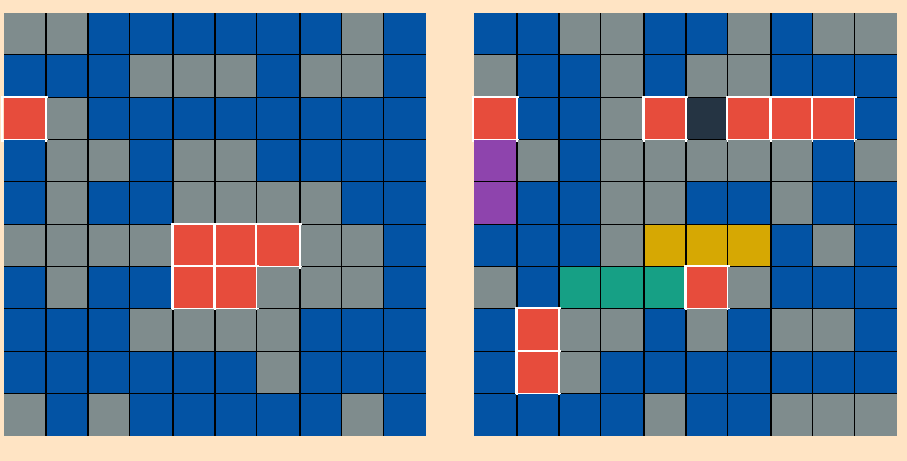
\includegraphics[width=\linewidth]{figuras/fig_fleet_board.png}
        \captionof{figure}{$10\times10$ board: 17 ship cells hidden among 100.}
        \label{fig:board}
    \end{minipage}
\end{center}
\end{column}
\begin{column}{0.46\textwidth}
\small
\textbf{PEAS} (Russell and Norvig):
\begin{itemize}\itemsep2pt
    \item \textbf{P}: shots needed to sink the fleet (fewer is better).
    \item \textbf{E}: partially observable, discrete, static, sequential.
    \item \textbf{A}: fire at one cell.
    \item \textbf{S}: hit / miss, and the notice that a ship sank.
\end{itemize}
\vspace{2mm}
Each agent shoots at \alert{its own board}: a game is a \alert{race} between two independent runs.
\end{column}
\end{columns}
\end{frame}

\begin{frame}{Three kinds of agents (Russell and Norvig)}
\begin{center}
    \begin{minipage}{0.92\textwidth}
        \centering
        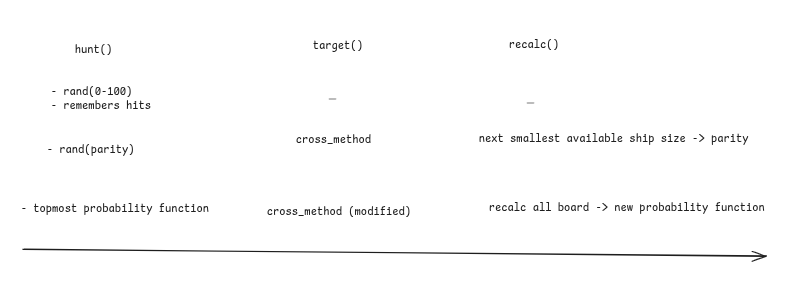
\includegraphics[width=\linewidth]{figuras/fig_agent_types.png}
        \captionof{figure}{Simple reflex, goal based and utility based, mapped to our three agents.}
        \label{fig:types}
    \end{minipage}
\end{center}
\vspace{-2mm}
\centering\scriptsize
\begin{tabular}{@{}lll@{}}
\toprule
\textbf{SRA} $\to$ simple reflex & \textbf{GBA} $\to$ goal based & \textbf{ABAOP} $\to$ utility based \\
condition--action rule & goal: sink the ship found & maximise a performance measure \\
\bottomrule
\end{tabular}
\end{frame}

%%%%%%%%%%%%%%%%%%%%%%%%%%%%%%%%%%%%%%%%%%%%%%%%%%%%%%%%%%%%%%%%%%%%%%%%%%%%%%%%
\section{The agents}

\begin{frame}{SRA: shoot at random (our baseline)}
\begin{columns}[T]
\begin{column}{0.5\textwidth}
\begin{center}
    \begin{minipage}{\textwidth}
        \centering
        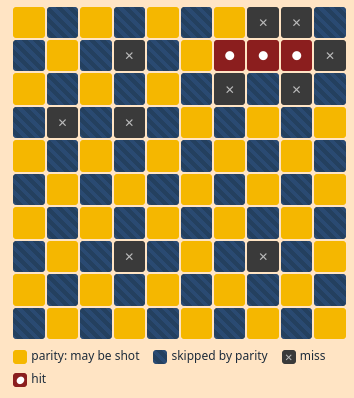
\includegraphics[width=\linewidth]{figuras/fig_sra_random.png}
        \captionof{figure}{Every cell not shot yet has probability $1/|U|$.}
        \label{fig:sra}
    \end{minipage}
\end{center}
\end{column}
\begin{column}{0.48\textwidth}
It ignores what it learns, so its behaviour has a \alert{closed form}: with $N=100$ cells and $K=17$ ship cells,
\[ P(X=m)=\frac{\binom{m-1}{K-1}}{\binom{N}{K}} \]
\vspace{-4mm}
\[ E[X]=\frac{K(N+1)}{K+1}=95.39 \]
\vspace{-2mm}
\begin{itemize}\small
    \item It needs almost the whole board.
    \item It needs all 100 shots in 17\,\% of the games (also reported by Berry).
    \item We use it to \alert{validate the simulator}.
\end{itemize}
\end{column}
\end{columns}
\end{frame}

\begin{frame}{GBA: parity search + directed sinking}
\begin{columns}[T]
\begin{column}{0.56\textwidth}
\begin{center}
    \begin{minipage}{\textwidth}
        \centering
        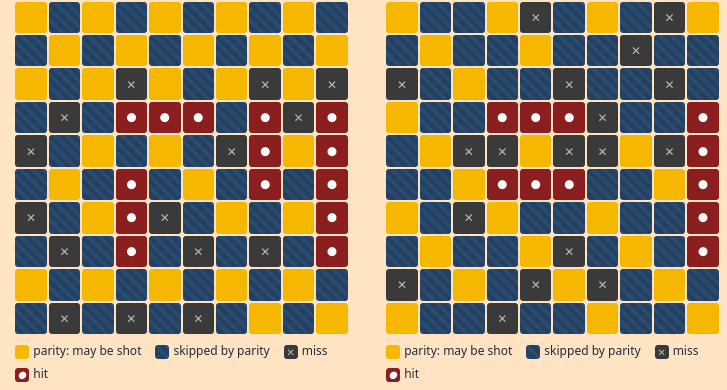
\includegraphics[width=\linewidth]{figuras/fig_gba_parity.png}
        \captionof{figure}{Parity $p=2$ (50 cells) and $p=3$ (34 cells).}
        \label{fig:parity}
    \end{minipage}
\end{center}
\end{column}
\begin{column}{0.42\textwidth}
\small
\textbf{Hunt.} Only cells with $(r-c)\bmod p=0$, where $p$ is the shortest ship afloat: \alert{no ship can hide} from that set (Berry).

\vspace{2mm}
\textbf{Target.} From the hit it explores Up--Right--Down--Left, \alert{locks the axis} at the first new hit, advances until a miss, then returns to the origin.

\vspace{2mm}
Our variation follows the \alert{line} of the ship instead of walking around every hit.
\end{column}
\end{columns}
\end{frame}

\begin{frame}{ABAOP: fire at the most probable cell}
\begin{columns}[T]
\begin{column}{0.52\textwidth}
\begin{center}
    \begin{minipage}{\textwidth}
        \centering
        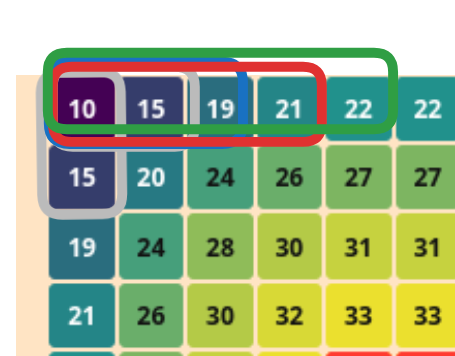
\includegraphics[width=\linewidth]{figuras/fig_abaop_density.png}
        \captionof{figure}{Density map: how many legal placements cover each cell.}
        \label{fig:density}
    \end{minipage}
\end{center}
\end{column}
\begin{column}{0.46\textwidth}
\small
For every ship afloat and every legal placement $\pi$,
\[ w(\pi)=\begin{cases}1 & \text{hunt}\\[-1mm] 10^{\,h(\pi)} & \text{target}\end{cases} \]
\vspace{-3mm}
\[ D(c)=\sum_{c\,\in\,\pi\ \text{legal}} w(\pi) \]
and it shoots at $\arg\max D(c)$ (Berry; popularised by Vsauce2).

\vspace{2mm}
No hand-made rules: the parity, the neighbours and the change of direction \alert{emerge from one formula}.
\end{column}
\end{columns}
\end{frame}

%%%%%%%%%%%%%%%%%%%%%%%%%%%%%%%%%%%%%%%%%%%%%%%%%%%%%%%%%%%%%%%%%%%%%%%%%%%%%%%%
\section{The application}

\begin{frame}{The application: watch the agent think}
\begin{columns}[T]
\begin{column}{0.66\textwidth}
\begin{center}
    \begin{minipage}{\textwidth}
        \centering
        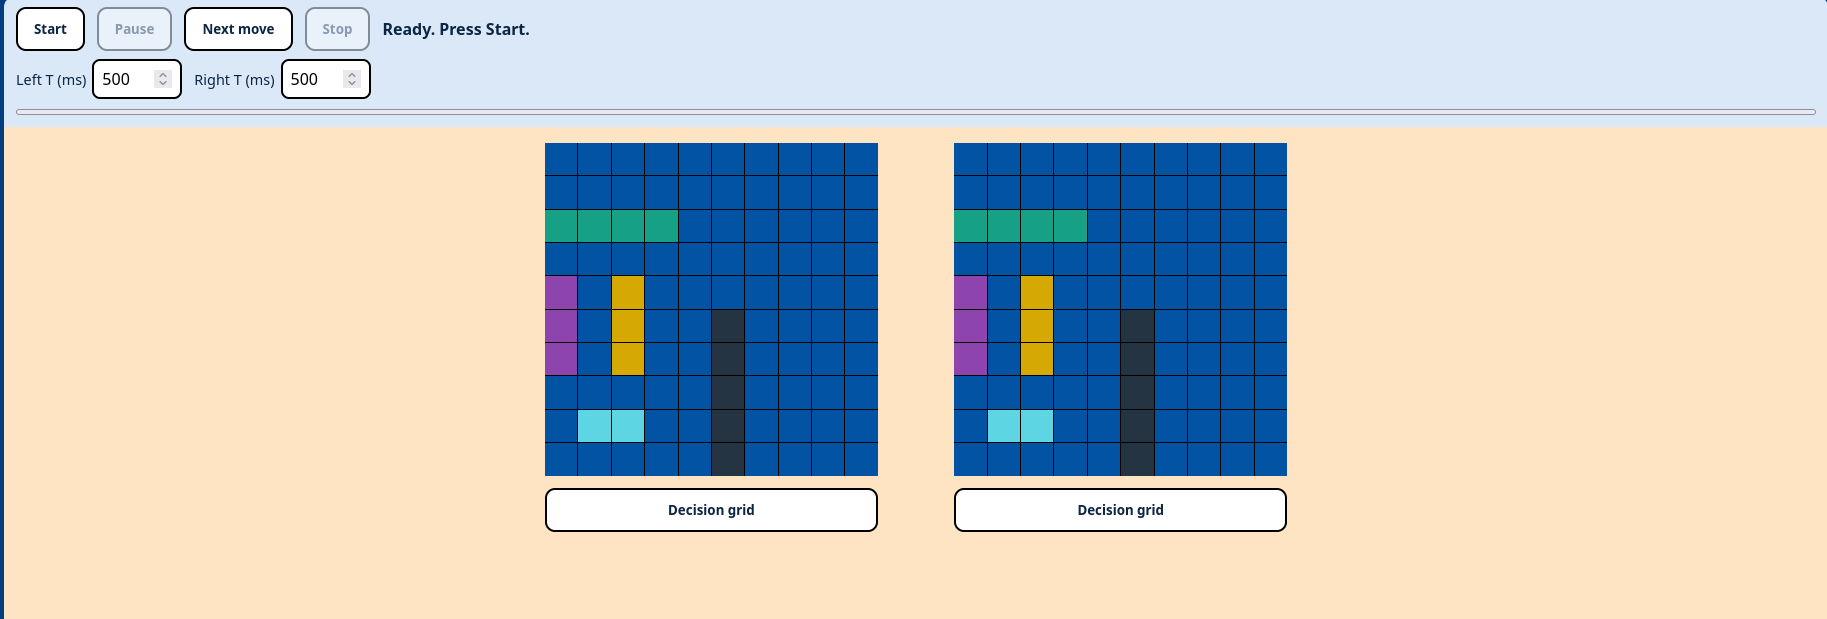
\includegraphics[width=\linewidth]{figuras/fig_app_game_desktop.png}
        \captionof{figure}{Boards and \emph{decision grids}: parity (GBA) and density (ABAOP).}
        \label{fig:app}
    \end{minipage}
\end{center}
\end{column}
\begin{column}{0.32\textwidth}
\begin{center}
    \begin{minipage}{\textwidth}
        \centering
        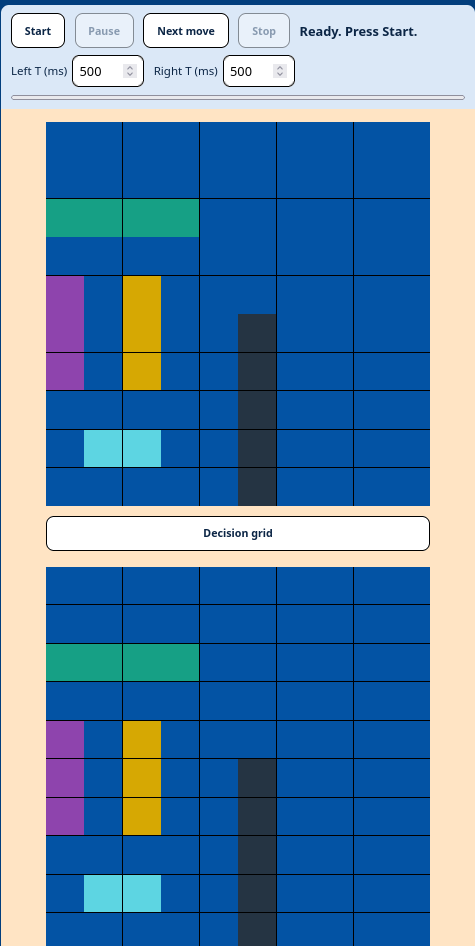
\includegraphics[width=\linewidth]{figuras/fig_app_phone.png}
        \captionof{figure}{Responsive: it also runs on a phone.}
        \label{fig:phone}
    \end{minipage}
\end{center}
\end{column}
\end{columns}
\vspace{-1mm}
\centering\small
JavaScript + HTML + CSS on GitHub Pages $\cdot$ \emph{Next move} step by step $\cdot$ delay $T$ live $\cdot$ $T=0$: 10\,000 games and a CSV.
\end{frame}

%%%%%%%%%%%%%%%%%%%%%%%%%%%%%%%%%%%%%%%%%%%%%%%%%%%%%%%%%%%%%%%%%%%%%%%%%%%%%%%%
\section{Results}

\begin{frame}{How we made the comparison fair}
\begin{columns}[T]
\begin{column}{0.46\textwidth}
\textbf{7 contests $\times$ 10\,000 games = 70\,000 games}
\vspace{2mm}
\begin{enumerate}\small\itemsep3pt
    \item \alert{Same fleet layout} for both agents: the difference is the agent, not the luck of the layout.
    \item \alert{The first shooter alternates}: on a tie the first to shoot wins, and that bias has to cancel.
    \item \alert{The loser plays out}: otherwise its shots are cut short and its average is biased.
\end{enumerate}
\end{column}
\begin{column}{0.5\textwidth}
\centering\scriptsize
\begin{tabular}{@{}clc@{}}
\toprule
\# & Contest & Layout \\
\midrule
1 & SRA vs SRA & same \\
2 & SRA vs SRA & \emph{different} \\
3 & GBA vs GBA & same \\
4 & ABAOP vs ABAOP & same \\
5 & SRA vs GBA & same \\
6 & SRA vs ABAOP & same \\
7 & GBA vs ABAOP & same \\
\bottomrule
\end{tabular}
\vspace{3mm}

\footnotesize Data integrity: 100\,\% of the 70\,000 records consistent.
\end{column}
\end{columns}
\end{frame}

\begin{frame}{How many shots does each agent need?}
\begin{columns}[T]
\begin{column}{0.56\textwidth}
\begin{center}
\begin{tikzpicture}
    \begin{axis}[battle, height=4.6cm, xlabel={Shots to sink the whole fleet}, ylabel={Fraction of games},
                 xmin=15, xmax=100, ymin=0, ymax=0.185, legend pos=north west]
        \addplot[cSRA]   table[x=shots, y=SRA]{data/dist_agents.csv};
        \addplot[cGBA]   table[x=shots, y=GBA]{data/dist_agents.csv};
        \addplot[cABAOP] table[x=shots, y=ABAOP]{data/dist_agents.csv};
        \addplot[black, dashed] table[x=shots, y=SRA_theory]{data/dist_agents.csv};
        \legend{SRA, GBA, ABAOP, SRA theory}
    \end{axis}
\end{tikzpicture}
\end{center}
\end{column}
\begin{column}{0.42\textwidth}
\centering\small
\begin{tabular}{@{}lcc@{}}
\toprule
Agent & Mean $\pm$ sd & Median \\
\midrule
SRA   & $95.4\pm4.8$ & 97 \\
GBA   & $50.3\pm8.7$ & 51 \\
ABAOP & $44.7\pm9.2$ & 44 \\
\bottomrule
\end{tabular}
\vspace{3mm}

\footnotesize
\begin{itemize}\itemsep2pt
    \item GBA saves \alert{47\,\%} of the shots of the SRA; ABAOP \alert{53\,\%}.
    \item The SRA matches its theory ($\chi^2$, $p=0.68$): the simulator is correct.
\end{itemize}
\end{column}
\end{columns}
\end{frame}

\begin{frame}{Who wins? The better agent still loses 1 game in 3}
\begin{columns}[T]
\begin{column}{0.54\textwidth}
\begin{center}
\begin{tikzpicture}
    \begin{axis}[battle, height=4.6cm, xmode=log, xlabel={Games played}, ylabel={Shots GBA $-$ shots ABAOP},
                 ymin=-4, ymax=16, title={GBA vs ABAOP: difference in shots, 95\,\% CI}]
        \addplot[name path=lo, draw=none] table[x=n, y=diff_lo]{data/running_gba_abaop.csv};
        \addplot[name path=hi, draw=none] table[x=n, y=diff_hi]{data/running_gba_abaop.csv};
        \addplot[fill=gray!30, draw=none] fill between[of=lo and hi];
        \addplot[black] table[x=n, y=diff]{data/running_gba_abaop.csv};
        \addplot[cABAOP, dashed, samples=2, domain=1:10000] {0};
    \end{axis}
\end{tikzpicture}
\end{center}
\end{column}
\begin{column}{0.44\textwidth}
\small
\begin{itemize}\itemsep3pt
    \item ABAOP vs GBA: \alert{67.0\,\%} of wins (CI 66.1--67.9), \alert{$5.36\pm0.24$} shots fewer per game.
    \item SRA won \alert{1 of 20\,000} games against them.
    \item Same kind vs same kind: $\approx$50\,\% each, as expected.
    \item The advantage is real but small against the noise of one game: 5 shots, sd of 12.5.
\end{itemize}
\end{column}
\end{columns}
\end{frame}

\begin{frame}{What does the intelligence cost?}
\begin{columns}[T]
\begin{column}{0.44\textwidth}
\begin{center}
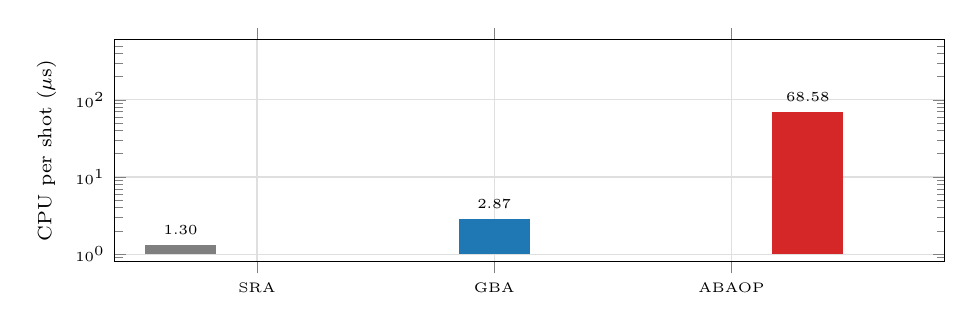
\begin{tikzpicture}
    \begin{axis}[battle, height=4.4cm, ybar, ymode=log, ymin=0.8, ymax=600, xmin=-0.6, xmax=2.9,
                 xtick={0,1,2}, xticklabels={SRA,GBA,ABAOP}, ylabel={CPU per shot ($\mu$s)},
                 bar width=0.9cm, point meta=explicit symbolic,
                 nodes near coords, nodes near coords style={font=\tiny}]
        \addplot[fill=cSRA,   draw=none] coordinates {(0,1.30) [1.30]};
        \addplot[fill=cGBA,   draw=none] coordinates {(1,2.87) [2.87]};
        \addplot[fill=cABAOP, draw=none] coordinates {(2,68.58) [68.58]};
    \end{axis}
\end{tikzpicture}
\end{center}
\end{column}
\begin{column}{0.54\textwidth}
\centering\scriptsize
\begin{tabular}{@{}lccc@{}}
\toprule
Agent & Per shot & Per game & Complexity \\
\midrule
SRA   & 1.30\,$\mu$s  & 0.12\,ms & $O(1)$ \\
GBA   & 2.87\,$\mu$s  & 0.14\,ms & $O(1)$ + recalc \\
ABAOP & 68.58\,$\mu$s & 3.07\,ms & $\Theta(N\,S)$ \\
\bottomrule
\end{tabular}
\vspace{3mm}

\footnotesize
\begin{itemize}\itemsep2pt
    \item ABAOP rebuilds the whole map every shot: $\approx$1\,449 cell checks ($N$ cells $\times$ fleet length $S$).
    \item 53$\times$ the cost of the SRA \dots but still only 3\,ms per game.
\end{itemize}
\end{column}
\end{columns}
\end{frame}

\begin{frame}{Our numbers against the authors}
\centering
\begin{tabular}{@{}lccc@{}}
\toprule
Median shots & Berry (DataGenetics, 2011) & Schwartz (2022) & \textbf{Our result} \\
\midrule
Random (SRA)          & 97 & 97 & \textbf{97} \\
Hunt/target + parity (GBA) & 64 & --- & \textbf{51} \\
Probability density (ABAOP) & 42 & 42 & \textbf{44} \\
\bottomrule
\end{tabular}
\vspace{4mm}

\begin{columns}[T]
\begin{column}{0.48\textwidth}
\small\textbf{Where we agree.} The random agent reproduces the published value exactly, and our density agent lands within two shots of Berry's.
\end{column}
\begin{column}{0.48\textwidth}
\small\textbf{Where we differ.} Our GBA beats the published hunt/target by \alert{13 shots}, because it follows the \emph{line} of the ship instead of walking around every hit.
\end{column}
\end{columns}
\end{frame}

%%%%%%%%%%%%%%%%%%%%%%%%%%%%%%%%%%%%%%%%%%%%%%%%%%%%%%%%%%%%%%%%%%%%%%%%%%%%%%%%
\section{Conclusions}

\begin{frame}{Conclusions}
\small
\begin{itemize}\itemsep3pt
    \item \textbf{ABAOP is the best agent}: 44.7 shots, 67\,\% of wins against the GBA. \emph{But} it wins two games out of three, not all of them: in a single game luck is still important.
    \item \textbf{GBA is the best balance}: it gets 88\,\% of the benefit for 4\,\% of the cost. For a bigger board, a phone, or thousands of decisions per second, it is the reasonable choice.
    \item \textbf{Is the ABAOP worth it?} Yes here: 3\,ms per game is nothing. The step SRA$\to$GBA saves 45 shots almost for free; the step GBA$\to$ABAOP saves 5.6 more and costs a thousand times more per shot saved.
    \item \textbf{The design of the experiment matters as much as the agent}: the same layout, the alternating first shooter and letting the loser finish were needed to avoid biased numbers.
    \item \textbf{Validation}: the SRA agrees with its closed form ($p=0.68$), which is what lets us trust the rest of the numbers.
\end{itemize}
\end{frame}

\begin{frame}{References}
\scriptsize
\begin{thebibliography}{9}
    \bibitem{berry2011} N. Berry, ``Battleship,'' \emph{DataGenetics}, Dec. 2011. [Online]. Available: \texttt{datagenetics.com/blog/december32011/}
    \bibitem{schwartz2022} A. Schwartz, ``Coding an intelligent Battleship agent,'' \emph{Towards Data Science}, 2022.
    \bibitem{vsauce2019} Vsauce2, ``The Battleship algorithm,'' YouTube, 2019.
    \bibitem{russell2021} S. Russell and P. Norvig, \emph{Artificial Intelligence: A Modern Approach}, 4th ed. Pearson, 2021.
    \bibitem{cormen2022} T. H. Cormen \emph{et al.}, \emph{Introduction to Algorithms}, 4th ed. MIT Press, 2022.
\end{thebibliography}
\end{frame}

\begin{frame}[standout]
Questions?\\[3mm]
{\normalsize\texttt{https://theuniquefersa.github.io/AI-Lab\_1-Agents/}}
\end{frame}

%%%%%%%%%%%%%%%%%%%%%%%%%%%%%%%%%%%%%%%%%%%%%%%%%%%%%%%%%%%%%%%%%%%%%%%%%%%%%%%%
%  BACKUP SLIDES: not presented, only in case of a question from the professor.
%%%%%%%%%%%%%%%%%%%%%%%%%%%%%%%%%%%%%%%%%%%%%%%%%%%%%%%%%%%%%%%%%%%%%%%%%%%%%%%%
\appendix

\begin{frame}{Backup: advantage of the first shooter}
\centering\small
On a tie the agent that shot first wins, so
\[ P(\text{first shooter wins}) = \frac{1+P(\text{tie})}{2} \]
\vspace{-2mm}
\begin{tabular}{@{}lccc@{}}
\toprule
Contest & $P(\text{tie})$ & Predicted & Observed \\
\midrule
SRA vs SRA     & 9.84\,\% & 54.92\,\% & 53.80\,\% \\
GBA vs GBA     & 3.29\,\% & 51.64\,\% & 51.25\,\% \\
ABAOP vs ABAOP & 4.34\,\% & 52.17\,\% & 52.87\,\% \\
SRA vs ABAOP   & 0.00\,\% & 50.00\,\% & 50.00\,\% \\
\bottomrule
\end{tabular}
\vspace{2mm}

\footnotesize That is why the first shooter has to alternate: otherwise one side starts with up to 5 points of advantage.
\end{frame}

\begin{frame}{Backup: does the fleet layout matter?}
\begin{columns}[T]
\begin{column}{0.56\textwidth}
\begin{center}
\begin{tikzpicture}
    \begin{axis}[battle, height=4.4cm, xlabel={$d=S^A-S^B$ (shots)}, ylabel={Fraction of games},
                 xmin=-30, xmax=30, ymin=0, legend style={at={(0.97,0.97)}, anchor=north east}]
        \addplot[cSRA, very thick]     table[x=d, y=same]{data/hist_diff.csv};
        \addplot[black, dashed, thick] table[x=d, y=different]{data/hist_diff.csv};
        \addplot[cABAOP]               table[x=d, y=abaop]{data/hist_diff.csv};
        \legend{{SRA, same layout}, {SRA, different layouts}, {ABAOP, same layout}}
    \end{axis}
\end{tikzpicture}
\end{center}
\end{column}
\begin{column}{0.42\textwidth}
\small
\begin{itemize}\itemsep3pt
    \item For the \textbf{SRA} the layout changes nothing ($\rho=0.03$): the two curves overlap.
    \item For the \textbf{ABAOP} the layout explains 29\,\% of the variance ($\rho=0.29$): some layouts really are harder for it.
    \item Using the same layout reduces the variance of the comparison by a factor of 1.41.
\end{itemize}
\end{column}
\end{columns}
\end{frame}

\begin{frame}{Backup: when does each ship sink?}
\begin{columns}[T]
\begin{column}{0.56\textwidth}
\begin{center}
\begin{tikzpicture}
    \begin{axis}[battle, height=4.6cm, xlabel={Ship sunk (in order)}, ylabel={Mean shot number},
                 xtick={1,2,3,4,5}, xmin=0.8, xmax=5.2, ymin=0, ymax=100, legend pos=north west]
        \addplot[cSRA,   mark=*]         table[x=k, y=SRA]{data/timeline.csv};
        \addplot[cGBA,   mark=square*]   table[x=k, y=GBA]{data/timeline.csv};
        \addplot[cABAOP, mark=triangle*] table[x=k, y=ABAOP]{data/timeline.csv};
        \legend{SRA, GBA, ABAOP}
    \end{axis}
\end{tikzpicture}
\end{center}
\end{column}
\begin{column}{0.42\textwidth}
\small
\begin{itemize}\itemsep3pt
    \item The ABAOP builds its advantage between the \alert{second and the fourth ship}.
    \item For the \alert{last ship} both agents need the same: the remaining empty area has to be searched anyway.
    \item Hit rate: SRA 17.9\,\%, GBA 35.0\,\%, ABAOP 39.7\,\%.
\end{itemize}
\end{column}
\end{columns}
\end{frame}

\end{document}
